\section{Theoretical Background}\label{sec:basics}
This section gives an overview of the \ac{NLI}, thetask that is used within this work. We also explain the architeecture of the model, that is used within most experiments and define lexical relations, that play an important role within this thesis.
\subsection{Natural Language Inference}\label{sec:basics_nli}
\ac{NLI} \citep{bowman2015large} deals with the problem to identify, whether one piece of natural text, namely the \textit{hypothesis}, can be inferred from another piece of text, namely the \textit{premise}. The hypothesis, in the remainder of this thesis denoted as $h$, is said to be entailed by the premise, denoted as $p$, if a human reader would conclude, that $h$ is true, given the fact that the $p$ is true. This definition differes from strict logical inference in the following way: While in \ac{NLI} \textit{a high plausability} for the $p$ to imply the $h$, based on the human judgement, is sufficient, the strict logical inference strives to achieve \textit{certainity} \citep{dagan2009recognizing}. \ac{NLI} essentially breaks down to an alignment problem \citep{maccartney2008phrase}, shown in the following example. Given the sentence pair
\begin{center}
\begin{tabular}{rl}
\textbf{Premise:} & Donald Trump is having a conversation in his living room. \\
\textbf{Hypothesis:} & The president of the United States is talking to people in the White House. 
\end{tabular}
\end{center}
the model is required to correctly align ``Donald Trump'' with ``The president of the United States'', ``having a conversation'' with ``talking to people'' and have information, that his ``bedroom'' is within the ``White House''. Here it can be seen, how the system would not only need to cope with different ways of expressing the same meaning, due to the nature of language, but also is required to access and process factual information, that is commonly known to an average human. Following \cite{bowman2015large}, the sentence relation can be classified using one out of three labels, \textit{entailment}, \textit{neutral}, \textit{contradiction}. Examples, taken from the SNLI Leaderboard\footnote{\href{https://nlp.stanford.edu/projects/snli/}{https://nlp.stanford.edu/projects/snli/}}, for each label are shown in Table \ref{tab:label_examples}.
\begin{table}[tph!]
\centering
\begin{tabular}{lc}
\textbf{Sentence-pair} & \textbf{Gold Label} \\
\toprule
\specialcell{A soccer game with multiple males playing.\\Some men are playing sport.} & entailment \\
\midrule
\specialcell{An older and younger man smiling.\\Two men are smiling and laughing at the cats, playing on the floor.} & neutral \\
\midrule
\specialcell{A man inspects the uniform of a figure in some East Asian country.\\The man is sleeping.} & contradiction\\
\bottomrule
\end{tabular}
\caption{Example sentence-pairs for each possible label, taken from \href{https://nlp.stanford.edu/projects/snli/}{SNLI Leaderboard}}.
\label{tab:label_examples}
\end{table}
If a human can infer that $h$ is very likely to be true, given the fact that $p$ is true, the gold label is entailment. In the first example, the hypothesis describes men ``playing sport'', which amongs other includes playing the ``soccer game'', and thus definetly still holds. In the second sentence pair, both sentences describe two smiling man, however the hypothesis adds information, that they are smiling ``at the cats''. While this new information may be true, it only is one of many potential scenarios and unkown, given the premise, thus the sample is labelled as neutral. Ih $h$ cannot be true if $p$ is true, the label is contradiction. In the last example, obviously the man cannot ``inspect'' anything and ``sleep'' at the same time, thus the labelling as contradiction.

\subsubsection{Relatedness to other NLP tasks}
While \ac{NLI} clearly is central to computational reasoning capabilities, as it detects the inference relationship between two texts, it is also very fundamental and applicable to a large variety of \ac{NLP} tasks, as the ability to recognize textual entailment is a fundamental and necessary problem towards real \ac{NLU} \citep{maccartney2007natural,bos2005recognising} in general. Many \ac{NLP} applications such as \ac{QA}, Summarization or \ac{IE} implicitly depend on this ability, as the huge variability of possible expressions for the same meaning it is a core phenomen of natural language \citep{dagan2009recognizing}. All three tasks require the model to infer, that the target meaning of interest can be inferred from corresponding other variants, consisting of a different textual expression. For \ac{QA} this is related to the identification of a correct answer. For summarization, on the one hand, the complete summary needs to be implied by the original text, on the other hand redundant sentences expressing the same meaning, thus one impying the other, should be ommited. Similarily \ac{IE}, especially if using multiple documents, needs to infer, whether two variants of text contain the same information, thus sentences entailing each other, or not. Even simple paraphrasing can be broken down to a lexical inference problem with mutual entailment between $p$ and $h$. As end applications for \ac{NLP} in addition to \ac{NLU} need to solve another complicated machine-learning task, it is hard to compare and directly improve their \ac{NLU} capabilities. Thus, one of the main purposes of \ac{NLI}, being a very basic problem towards \ac{NLU}, is serving as a benchmark to directly improve \ac{NLU}, with any enhancement potentially helping a large variety of higher level tasks within \ac{NLP} \citep{williams2017broad,cooper1996using,bos2005recognising,dagan2006pascal}.  

\subsection{Lexical Semantic Relations}\label{sec:word_relations}
Lexical relations describe the relationship between words\footnote{While there is no single definition for \textit{word}, we use the term equivalent to a single token identified by typical tokenizers, thus it is defined by its surface form.}, whereas \textit{Lexical Semantic Relations} are a special form of lexical relations, consisting of relations, that refer to the meaning of the word \citep{murphy2003semantic}, which have shown to be helpful for detecting lexical inferences \citep{dagan2009recognizing}. We define those relations in this subsection based on the definition of \cite{Jurafsky2008May}. One key characteristic of natural language is ambiguity, which also is present in lexical semantics as words may have several meanings or \textit{senses}\footnote{The phenomen of words having multiple senses is called \textit{homonymy}, if both senses have no meaningful relation but still share the surface form like ``bank'' (financial institution) and ``bank'' (sloping mound). If those senses are semantically related like ``milk'' (take milk from female mammals) and ``milk'' (like cow's milk), the relationship is called \textit{polysemy} \citep{Jurafsky2008May}}. To deal with this phenomene, lexical semantic relations are defined between senses rather than words. For the sake of simplicity for the most part we follow a naive approach in the following chapters of assuming the most dominant sense of a word, when referring to it. Specifically we define \textit{Synonymy}, \textit{Antonomy}, \textit{Hypernomy} and \textit{Holonomy}, the latter two relations are visualized\footnote{This is for illustration purposes only and we only added some relevant relations between the entities, more relation are possible. For instance, the holonym relationship would of course hold between \textit{head} and any other \textit{animal}.} in Figure \ref{fig:lexical_resources}.
\begin{figure}[tph!]
\centering
	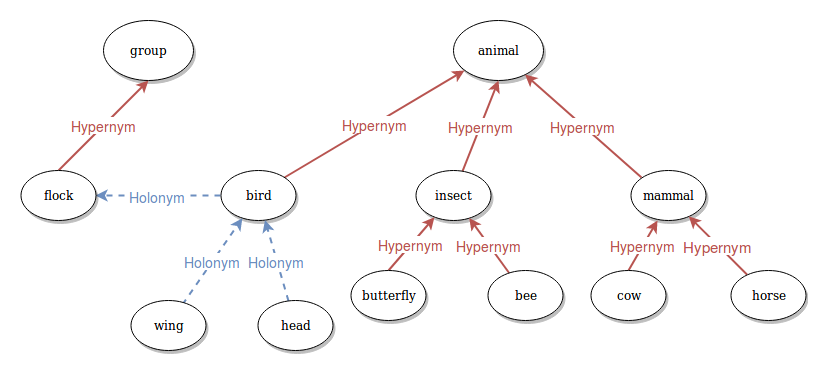
\includegraphics[totalheight=7cm]{fig/lexical_relations.png}
	\caption{A sample ontology of animals to illustrate the lexical relations \textit{Hypernomy} and \textit{Holonymy}.}
	\label{fig:lexical_resources}
\end{figure}
\subsubsection{Synonymy and antonomy}
Synonomy is a symmetric relationship between two senses or two words. Two senses of two different words are said to be synonyms, if they have the same or nearly the same meaning. Synonymy between words is holds, if one word can be replaced by the other word in any sentence  without changing the meaning of the sentence. True synonyms are rare, as most words at least have subtle differences in their meaning or are used within different contexts. We thus follow common practice and loosen the strict definition by refering to synonmys if they have approximately similar meanings. Like synonomy, antonomy is a symmetric relationship between senses. These senses however have the opposite meaning, which might be caused by a binary opposition like ``opened/closed'', by different ends on some scale like ``hot/cold'' or by directional change like ``upwards/downwards''. Since antonyms semantically are identical in all other aspects with synonyms, these relations are hard to distinguish from each other automatically.

\subsubsection{Hypernomy}
Hypernomy (or Hyponomy) is an asymmetric relation between two senses and also referred to as the \textit{is-a} relation. The more specific sense (e.g. ``bee'') is called the \textit{hyponym} of the more general sense (e.g. ``insect''), which is called \textit{hypernym}. \cite{Jurafsky2008May} give a formal definition for Hyponomy in terms of entailment: 
\begin{quotation}\noindent
``[...] a sense $A$ is a hyponym of a sense $B$ if everything that is $A$ is also $B$ and hence being an $A$ entails being a $B$, or $\forall x$ $A(x) \Rightarrow B(x)$.'' \citep{Jurafsky2008May}
\end{quotation}
In most cases, hypernomy is transitiv, thus if a ``cow'' is a hyponym of ``mammal'' and ``mammal'' is a hyponym of ``animal'', ``cow'' is also a hyponym of ``animal''. An important relation for this thesis holds between two words, sharing a close hypernym. In Figure \ref{fig:lexical_resources} for instance, ``bee'' and ``butterfly'' share the close hypernym ``insect'', we refer to them as \textit{co-hyponyms}.

\subsubsection{Holonomy}
Holonomy or Meronomy refers to the \textit{part-whole} relation. In the illustration of Figure \ref{fig:lexical_resources}, the ``wing'' is a part of a ``bird'' and a ``bird'' is a part of a ``flock''. We say that a ``bird'' is a \textit{meronym} of ``flock'', while ``flock'' is the \textit{holonym} of ``bird''. As opposed to Hypernyomy, this asymmetric relation is not generally transitiv. While a ``flock''\footnote{This is an example for polysemy, as \textit{flock} may refer to a group of birds, but also to a group of e.g. sheep. In this case we assume the sense of a group of birds and ignore other senses.} obviously consists of several birds, In this case ``birds'' is generally not replacable with ``heads'', even though ``head'' is a meronym of ``bird''. 
\subsubsection{Lexical semantic realtions for \ac{NLI}}
the introduced lexical semantic relations are far from complete. One may define many other relations that hold between two words, like for example \textit{president-of} can define the relationship between ``Donald Trump'' and ``USA''. Yet, the presented relations are well captured in various lexical knowledge bases, that will be explained in Section §\ref{sec:ext_resources}, and even though they only capture a small amount of the requirements for \ac{NLI}, identifying those relation amongst words of $p$ and $h$ is a crucial for the task \citep{shwartz2015learning}. Even though they exclude phenomenas like causality, at the very basic, a model for \ac{NLI} should identify that synonyms or hypernyms of a word cover the same meaning an thus can be inferred. While not always, similar indicators are given by meronyms, here however this may differ, depending on the sense itself or its context \citep{shwartz2015learning}. Meronyms for locations are usually covered by their holonym. For instance ``John is in \textit{Paris}'' implies ``John is in \textit{France}'', with ``Paris'' being a meronym, or \textit{part-of} ``France''. However for the example in figure \ref{fig:lexical_resources}, the opposite holds: ``A lion eats a \textit{flock}'' implies that the lion eats a ``bird''. As opposed to the locations, in this case, the holonym ``flock'' covers the meronym, not vice-versa. In the remainder of this thesis, we refer to the presented lexical semantic relations, applied on the entailment problem, when referring to \textit{lexical inference}.
\subsection{Shortcut-Stacked-Encoder and Residual Encoder}\label{sec:residual_encoder_def}
We conduct most of our experiments with the Shortcut-Stacked Encoder \citep{nie2017shortcut} and the recently adapted version to the Residual-Stacked Encoder. They achieve state-of-the-art results for two large datasets\footnote{These are explained in deeper detail in §\ref{sec:basics_datasets}} for \ac{NLI} and follow the Siamese Architeture, originally introduced by \cite{bromley1994signature}. Subsequentially, they first encode $p$ and $h$ individually, using the same sentence encoder with shared weights, into fixed length sentence representations and then predict the entailment label from the combination of both representations using an additional \ac{MLP}.

\subsubsection{Sentence Encoding for Shortcut-Stacked-Encoder}
The key novelty of this approach for \ac{NLI} is the way sentence representations are created using a three-layer \ac{biLSTM} with shortcut connections and row-wise max-pooling. An overview of this architecture is given in Figure \ref{fig:sentence_emcoder_shortcut}.
\begin{figure}[tph!]
\centering
	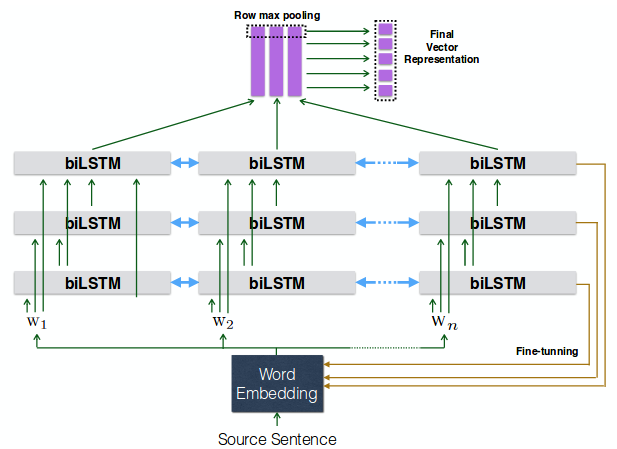
\includegraphics[totalheight=8cm]{fig/sentence_encoder_shortcut.png}
	\caption{The architecture of the sentence-encoding component within the Shortcut-Stacked-Encoder, taken from \cite{nie2017shortcut}.}
	\label{fig:sentence_emcoder_shortcut}
\end{figure}
Due to the arbitrary amount of words in textual input, a widely used strategy to encode variable length inputs to fixed length vectors is the usage of \ac{LSTM} \citep{hochreiter1997long} or the bi-directional variant \ac{biLSTM} \citep{graves2005framewise}. Essentially these components learn with the use of gates what information to keep and forget at a given point in time, meaning at a given word in sequential order within a sentence, when applied to text. By sequentially going through a sentence in one or two directions respectivly, these eural components are capable of exploiting word-order and take context of each word into account, when creating the compact sentence representation.
\newline

\noindent
The main difference of the Shortcut-Stacked Encoder to typical architectures, using a multi-layer \ac{biLSTM}, is, that the input to the \ac{biLSTM} in a following layer is not only the output of the previous layer (as commonly done), but the output of \textit{all} previous layers, together with the word embeddings. This is visualized within Figure \ref{fig:sentence_emcoder_shortcut} and referred to as ``Shortcut-connections'' \citep{nie2017shortcut}. Let $t$ denote the word position at the current time step within the input sentence, consisting of a total of $n$words. In the first step, the embedding layer maps each textual word $\omega_t$ with $t \in \mathbb{N}$ and $0 < t \\leq n$ of the source sentence $(\omega_1, \omega_2, ..., \omega_{n-1} \omega_n)$ to a $d$-dimensional word vector $w_t \in \mathbb{R}^d$. According to \cite{nie2017shortcut} we denote $x_t^i$ to be the input of the $i$th \ac{biLSTM} at timestep $t$. Naturally the input to the first layer are the word-embeddings itself, thus:
\begin{equation}
x_t^1 = w_t
\end{equation} 
In all \ac{biLSTM} with $i > 1$, the input is the concatenation of all intermediate inputs of previous layers at the timestep $t$, together with the initial word embeddings $w_t$. Let $[]$ denote the vector concatenation and $h^i_t$ be the output of the $i$th \ac{biLSTM} at timestep $t$. The input $x^i_t$ formally looks as follows:
\begin{equation}\label{eq:stacked_encoder_input}
x_t^i = [w_t, h_t^{i-1}, h_t^{i-2}, ... , h_t^1]
\end{equation}

\noindent
Only the last \ac{biLSTM} layer is used to generate the final sentence representation. Let $m$ be the amount of layers in total and $d_m$ be the hidden state dimensionality of the last layer, that is defined as $H_m=(h_1^m, h_2^m, ..., h_n^m)$, thus a matrix, consisting of all aligned outputs $h^t$ of the last layer. The final sentence representation $v$ is obtained by applying row-max-pooling over the last layer's output vectors:
\begin{equation}
v = max(H^m)
\end{equation}
With each $h_i^m \in \mathbb{R}^{2d_m}$ and $H^m \in \mathbb{R}^{2d_m \times n}$ the resulting sentence vector $v \in \mathbb{R}^{2d_m}$ essentiallly captures the highest value of each dimension over all timesteps\footnote{$d_m$ is multiplicated by $2$ since the \ac{biLSTM} creates $d_m$ features for going through the sentence forwards and backwards respectively.}. We strongly leverage from the max-pooled sentence representation in Section §\ref{sec:understanding} and discuss how this method can be exploited in the corresponding section in detail.
\subsubsection{Classification}
A two-layer \ac{MLP}, using \ac{ReLU} as activation function, and a final softmax-layer are used for the prediction. The input $m$ to the classifier is the concatention of the sentence representations $v_p$ and $v_h$ for $p$ and $h$ respectively, together with the element-wise difference and the element-wise product, denoted as $\otimes$, of both representations:
\begin{equation}
m = [v_p, v_h, |v_p-v_h|, v_p \otimes v_h]
\end{equation}
Even though a \ac{MLP} theoretically would be able to learn the latter two features, \cite{mou2015natural} showed that this particular feature concatenation gives a performance gain for neural models for \ac{NLI}.
\subsubsection{Training}
For all our reimplementations, using pytorch\footnote{\href{http://pytorch.org/}{http://pytorch.org/}}, of the model we follow the parameters of the original paper of \cite{nie2017shortcut}. The model is trained using Adam \citep{kingma2014adam} parameter optimization, cross-entropy loss as objective function and minibatches of size 32. To avoid overfitting a dropout of 0.1 is applied on each layer of the \ac{MLP} and the accuracy is evaluated on a regular basis on a different dataset than the train data, the development set, as it is common practice in machine learning. The final performance is estimated by evaluating the best model based on the accuracy on the development set on unseen hold-out data, the test set. 300-dimensional GloVe 840B pretrained word-embeddings \citep{pennington2014glove} are used and fine-tuned during training. Three additional word-vectors are added, one for unknown words, as well as one to indicate the start and one to indicate the end of a sentence. The learning rate starts with 0.0002 and is reduced by half every second iteration. We conduct our experiments with different re-implementations of this model, partly due to reduce training time by reducing the dimensionality of the components, partly due to changes within the original paper.
\subsubsection{Residual Encoder and Reimplementation Variants}
In a second version of the same paper, \cite{nie2017shortcut} introduced the Residual-Stacked Encoder, slightly adapting the way sentences are encoded. Creating the input to the $i$th \ac{biLSTM} layer $x_t^i$ by concatenating all previous outputs $(h_t^{i-1}, h_t^{i-2}, ... , h_t^1)$ together with $w_t$, naturally leads to a tremendous increase of parameters with an increasing amount of layers. By using residual connections, instead of concatenating all previous outputs, previous outputs are summed up instead of being concatenated, thus equation (\ref{eq:stacked_encoder_input}) changes to
\begin{equation}
x_t^i = [w_t, h_t^{i-1} + h_t^{i-2} + ... + h_t^1]
\end{equation}
and reduces the parameter size.
\paragraph*{Implementation Variants}
We use the following implementations of the model. The performance comparison between the models based on SNLI\footnote{SNLI is a huge dataset for \ac{NLI} and will be explained in §\ref{sec:basics_datasets}}, is listed in Table \ref{table:reimplementation_performance} and do not differ tremendously from what \cite{gong2017natural} estimated to be the human performance on the same task.
\begin{table}[!htbp]
\begin{center}
\begin{tabular}{lccc}
\textbf{Model} & \textbf{SNLI train acc.} & \textbf{SNLI dev acc.} & \textbf{SNLI test acc.}\\
\toprule
Shortcut-Stacked Encoder\textsuperscript{$\dagger$} & 87.4\% & 85.2\% & 84.8\% \\
Shortcut-Stacked Encoder\textsuperscript{$\dagger\dagger$} & 89.4\% & 86.0\% & 85.4\% \\
Residual Encoder\textsuperscript{$\dagger$} & 91.1\% & 85.9\% & 85.8\% \\
Residual Encoder\textsuperscript{$\Diamond$} & 91.0\% & 87.0\% & 86.0\% \\
\midrule
Human Performance \citep{gong2017natural} & - & - & 87.7 \\
\bottomrule
\end{tabular}
\caption{Accuracy in percent of different implementations of the model from \cite{nie2017shortcut}, achieved on the SNLI dataset compared with human performance.}
\label{table:reimplementation_performance}
\end{center}
\end{table}
\begin{itemize}
\item We refer to Shortcut-Stacked Encoder\textsuperscript{$\dagger$} as the first re-implementation with reduced parameter size w.r.t. the original proposed model. This uses $256\times2$, $512\times2$ and $1024\times2$ dimensions for the three layers of the sentence encoding \ac{biLSTM} and $1600$ dimensions in the classifier \ac{MLP}.
\item We refer to Shortcut-Stacked Encoder\textsuperscript{$\dagger\dagger$} as the the same re-implementation using the full parameters, as reported originally. This uses $512\times2$, $1024\times2$ and $2048\times2$ dimensions for the three layers of the sentence encoding \ac{biLSTM} and $1600$ dimensions in the classifier \ac{MLP}.
\item We refer to Residual Encoder\textsuperscript{$\dagger$} when we use our own re-implementation with residual connections. The sentence-encoding \ac{biLSTM}s each have the dimensionality of $600\times2$ and the layers of the \ac{MLP} of $800$.
\item We refer to Residual Encoder\textsuperscript{$\Diamond$} when we use the final published version of \cite{nie2017shortcut} with their provided code\footnote{https://github.com/easonnie/ResEncoder}. This model has the same parameter sizes as Residual Encoder\textsuperscript{$\dagger$}.
\item We refer to the plain model name, when talking about the model structure in general.
\end{itemize}
